\subsection{Apparato di misura}
Gli strumenti principali a disposizione per questa esperienza (fatta eccezione per i soliti moduli \texttt{NIM}) consiste in:
\begin{itemize}
	\item una sorgente radioattiva principale di \co\! e altre sorgenti meno attive per la calibrazione: \cs, \na, \am;
	\item il PMT1: un rivelatore basato su uno scintillatore organico (che fungerà da bersaglio);
	\item il PMT2: un rivelatore basato su un cristallo scintillatore di NaI(Tl) 2"$\times$2" dotato di un preamplificatore in cascata al fotomoltiplicatore (che useremo come spettrometro);
	\item un formatore/amplificatore che produce in uscita un segnale gaussiano con altezza di picco proporzionale all'energia rilasciata e durata $\sim \SI{10}{\micro s}$;
	\item un ADC a 13 bit che può sia essere triggerata dall'esterno, sia campionare automaticamente sul picco tutti i segnali che superano una certa soglia interna\footnote{anche molto bassa CIPPALIPPA} (chiameremo questa modalità \emph{automatica}).
\end{itemize}

\subsubsection{Sorgenti radioattive}
La sorgente radioattiva principale di \co\; decade $\beta^-$ in uno stato eccitato di $^{60}$Ni che a sua volta decade $\gamma$ due volte in cascata emettendo fotoni di $\SI{1.17}{MeV}$ e $\SI{1.33}{MeV}$.

La sorgente ha un'attività dichiarata di \SI{74}{MBq} al febbraio 1997 e si trova in un contenitore di piombo con collimatore a sezione circolare\footnote{Di un materiale diverso e a Z più basso.}. 
Data l'emivita del \co\; di $\tau_2 = \SI{5.3}{yr}$ alla data della nostra esperienza l'attività stimata della sorgente è $\sim 2^{21/5.3} \cdot \SI{74}{MBq} = \SI{4.7}{MBq}$.

Dalla costante di dose del \co\;  ($\SI{0.35}{\micro Sv\;m^2\;MBq^{-1}\;h^{-1}}$) FONTE CIPPALIPPA è possibile stimare la dose assorbita nel corso dell'esperienza: $\SI{0.35}{\micro Sv\;m^2\;MBq^{-1}\;h^{-1}} \cdot \SI{4.7}{MBq} \cdot (\SI{1}{m})^2= \SI{1.6}{\micro Sv\;h^{-1}}$ (a un metro di distanza) che va confrontato con il fondo naturale $\sim\SI{0.3}{\micro Sv\;h^{-1}}$. Si tratta di una stima per eccesso poiché considera la sorgente isotropa, ma la nostra sorgente è schermata ed emette solo in un piccolo angolo solido (non nella nostra direzione).

Le altre sorgenti di calibrazione a disposizione hanno un'attività minore di $\SI{72}{kBq}$\footnote{Si tratta dell'attività dichiarata dalla ditta produttrice alla data di vendita che è ignota.}\marginpar{questo dettaglio non è particolarmente rilevante ma bho (Bob)} e i loro principali modi di decadimento sono schematizzati in \autoref{tab:sorgenti_cal}. Notiamo inoltre che il \na\; decade $\beta^+$, ci aspettiamo perciò di osservare nel suo spettro il segnale dei fotoni $\gamma$ a \SI{511}{keV} prodotti nell'annichilazione.

\begin{table}[h]
	\centering
	\begin{tabular}{cccc}
		\toprule
		sorgenti & \multicolumn{3}{c}{principali modi di decadimento} \\
		\midrule
		\co & $\beta^{-} (\SI{318}{keV})$ & $\gamma (\SI{1173}{keV})$ & $\gamma (\SI{1332}{keV})$  \\
		\cs & $\beta^{-} (\SI{512}{keV})$ & $\gamma (\SI{662}{keV})$ \\
		\na & $\beta^{+} (\SI{546}{keV})$ & $\gamma (\SI{1275}{keV})$ \\
		\am & $\alpha (\SI{5486}{keV})$ & $\gamma (\SI{59.5}{keV})$ \\
		\bottomrule
	\end{tabular}
	\caption{\label{tab:sorgenti_cal} Principali modi di decadimento delle sorgenti a disposizione FONTE CIPPLIPPA}
\end{table} 

\subsubsection{Schema dell'apparato sperimentale}
La strumentazione a disposizione è disposta come in \autoref{fig:schema_apparato}: il PMT1 si trova subito davanti al collimatore della sorgente di \co. Il PMT2 si trova su una base capace di ruotare attorno ad un perno che con ottima approssimazione si trova sulla verticale del bersaglio.
 \begin{figure}[h]
	\centering
	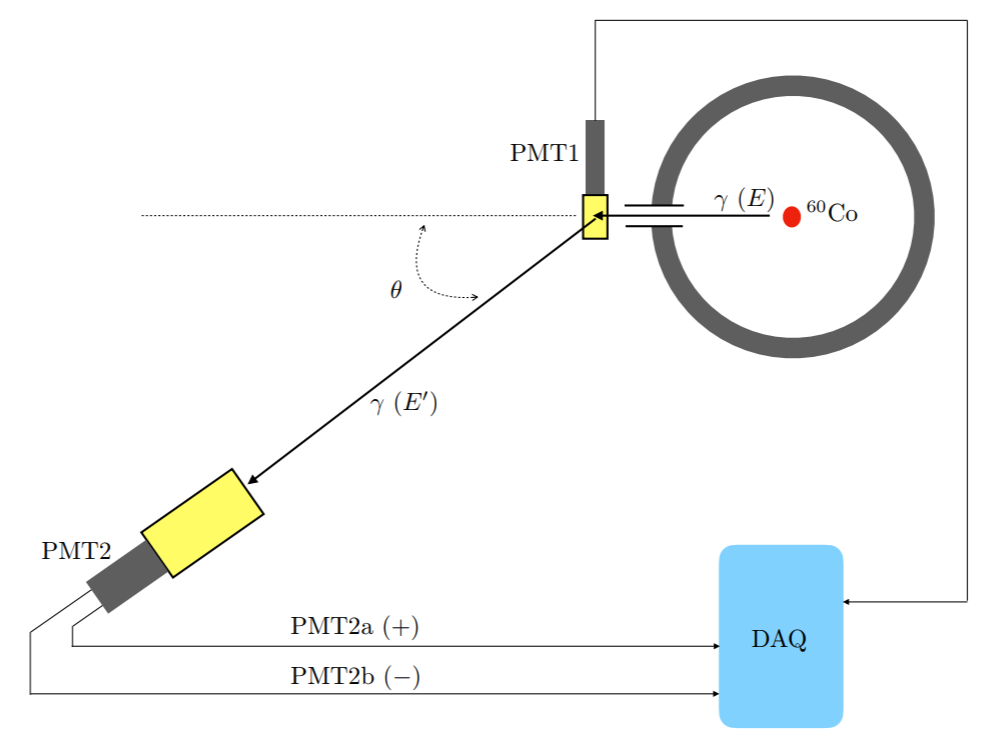
\includegraphics[width=25em]{schema_apparato}
	\caption{\label{fig:schema_apparato}Schema dell'apparato sperimentale}
\end{figure}

